%In the first exercise, the earthquake catalogue will be declustered and the time-variation in completeness analysed. For three of the sources shown in figure \ref{fig:KathGSHAPLabel} (Sources 8.CH.257, 8.CH.258 and 8.CH.259) the recurrence model will be calculated (first using the algorithm of \cite{KijkoSmit2012} - others could be attempted) and maximum magnitude inferred using one of the \cite{Kijko2004} methods 
%
%The configuration file indicates to the toolkit where to look for input files, write output files, which processes and methods to apply and any possible parameters that should be set for given methods. A ''comprehensive'' example of the configuration file is given automatically in the file \verb=config.yml=, which outlines all possible options. The easiest process is to open this file, then edit and delete various options and parameters before saving the configution file to a new file (e.g. \verb=my_config_1.yml=) then executing that in place of the original configuration file.    
%
%The various settings for the different algorithms will be discussed in due course, so the following considers just the main headers (i.e. the control) of the toolkit:
%
%\begin{Verbatim}[frame=single, commandchars=\\\{\}, fontsize=\scriptsize, samepage=false]
%\#*****************************************************************************
%\# HMTK Workflow Configuration File
%\#*****************************************************************************
%
%\#=============================================================================
%\# Input/Output Files
%\#=============================================================================
%
%\# Inputs the Path to the Earthquake Catalogue
%input_catalogue: input/NepalCatalogue_ISC.csv
%\# Inputs the path to the source model (if needed)
%input_model: input/Nepal_3GSHAP_sources.xml
%\# Inputs the path to the output directory
%output_directory: output/
%\# Plotting Folders
%figure_directory: output/plotting/
%
%
%\# Configuration for the Declustering Algorithm (leave blank if not wanted)
%declustering_config: \{\\
%    \# Algorithm choice\\
%    \# 'GardnerKnopoff'  | 'Afteran'\\
%    algorithm: 'GardnerKnopoff',\\
%    \# Choice of magnitude and distance scaling relations\\
%    \# 'GardnerKnopoff' | 'Uhrhammer' | 'Gruenthal'\\
%    time_distance_windows: 'GardnerKnopoff',\\
%    \# Foreshock time as a proportion of aftershock time\\
%    # (GardnerKnopoff only)
%    fs_time_prop: 0.0,\\
%    \# Fixed-width moving time window in days (Afteran only)
%    time_window=60.
%    \}\\
%
%
%\# Configuration for the Completeness Algorithm (only Stepp supported)
%completeness_config: \{
%    \# Choice of algorithm (currently only 'Stepp' supported)
%    algorithm: 'Stepp', 
%    \# Magnitude interval 
%    magnitude_bin: 1.0,
%    \# Time interval (years - as float)
%    time_bin: 5.0,
%    \# Locks the increment to ensure completeness values only increase for
%    \# longer periods 
%    \# True | False
%    increment_lock: True,
%    \# If a plot is wanted (i.e. for Stepp (1971) then set to true
%    include_plot: True,
%    \# If a pre-computed completeness is preferred, define here
%    completeness_table: \}
%
%
%recurrence_config: \{
%    \# Choice of algorithm
%    \# 'Weichert' | 'KijkoSmit' | 'MaxLikelihood'
%    algorithm: 'KijkoSmit',
%    \# Magnitude for calculating rate (if not set will return true a-value
%    reference_magnitude: ,
%    \# Magnitude bin interval
%    magnitude_interval: 0.1,
%    \# Minimum magnitude for sources
%    minimum_magnitude: 4.5\}
%
%
%mmax_config: \{
%    \# Choice of algorithm
%    \# 'KijkoSellevol' | 'KijkoSellevolBayes' | 'KijkoNonparametric | 
%    \# 'CumulativeMoment'
%    algorithm: 'KijkoNonparametric',
%    \# Minimum magniutde (for Kijko & Sellevol methods only)
%    input_mmin: 5.5,
%    \# Input maximum magnitude (if not specified will take largest in catalogue)
%    input_mmax: ,
%    \# Uncertainty on maximum magnitude
%    input_mmax_uncertainty: ,
%    \# Number of N largest earthquakes for consideration (KijkoNonparametric 
%    \# only)
%    number_earthquakes: 50,
%    \# Maximum number of iterations (for all Kijko methods)
%    max_iterations: 1000\}
%       
%\end{Verbatim}
%
%In the initial lines, the toolkit is told the path to look for the input earthquake catalogue (\verb=eq_catalog_file=); the path to which it should write the ''pre-processed catalogue'' (\verb=pprocessing_catalog_file=); the path to which it should write the completeness table, or from which it should read the completeness table if no completeness jobs are defined (\verb=completeness_table_file=); the path from which it should find the area source geometries (\verb=source_model_file=), formatted here as xml (\verb=source_model_file=), and the path to write the output area sources (\verb=result_file=). 
%
%The ''pre-processing'' refers to the combined operations for declustering and/or completeness - i.e. those that remove from consideration all events that are not indicative of complete stationary seismicity. If the user wishes to simply execute those jobs and no others then they should set the value \verb=apply_processing_jobs: no=. This will cause the program to terminate after completion of the pre-processing tasks. If the user has specified a valid path for the \verb=pprocessing_catalog_file= the program will export the catalogue with foreshocks, aftershocks and incomplete magnitude events removed.
%
%After completion of the ''pre-processing'' tasks, the toolkit will then undertake the ''processing'' tasks. These are the calculations to determine the parameters of the double-truncated \cite{GutenbergRichter1944} distribution (i.e. a-value, b-value, minimum magnitude and maximum magnitude). If no source model input is specified in the \verb=source_model_file=, the processing will return (to the screen) a single a-value, b-value, $m_max$ and their respective uncertainties for the whole catalogue. Otherwise the program will loop over each of the zones specified in the file, select those earthquakes from the pre-processed catalogue that are found inside each zone and calculate the recurrence parameters for each zone. The output will then be written to the \verb=result_file=.
%
%\textbf{The order in which the ''pre-processing'' and the ''processing'' tasks are define in the configuration is the order in which the program will execute them!}

\section{The Seismicity Tools}

The seismicity tools are intended for use in deriving activity rates from an observed earthquake catalogue, which may include both instrumental and historical seismicity. The tools are broken down into five separate libraries: i) Declustering, ii) Completeness, iii) Calculation of Gutenberg-Richter a- and b-value, iv) Statistical estimators of maximum magnitude from seismicity) and v) Smoothed Seismicity. In a common use case it is likely that many of the above methods, particularly recurrence and maximum magnitude estimation, may need to be applied to a selected sub-catalogue (e.g. earthquakes within a particular polygon). The toolkit allows for the creation of a source model containing one or more of the supported OpenQuake seismogenic source typologies, which can be used as a reference for selection, e.g. events within an area source (polygon), events within a distance of a fault etc. The supported input formats for both the catalogue and the source model are described below. 

\subsection{The Catalogue Format and Class}

The input catalogue must be formatted as a comma-separated value file (.csv), with the following attributes in the header line (attributes with an * indicate essential attributes), although the order of the columns need not be fixed:

\begin{table}
\begin{tabular}{|l|l|}  \hline 
Attribute & Description \\ \hline
eventID* & A unique identifier (integer) for each earthquake in the catalogue \\
Agency & The code (string) of the recording agency for the event solution  \\
year* & Year of event (integer) in the range -10000 to present \\
 & (events before common era (BCE) should have a negative value)\\
month* & Month of event (integer)\\
day* & Day of event (integer) \\
hour* & Hour of event (integer) - if unknown then set to 0 \\
minute* & Minute of event (integer) - if unknown then set to 0 \\
second* & Second of event (float) - if unknown set to 0.0 \\
timeError & Error in event time (float) \\
longitude* & Longitude of event, in decimal degrees (float) \\
latitude* & Latitude of event, in decimal degrees (float) \\
SemiMajor90 & Length (km) of the semi-major axis of the 90 \% \\
            & confidence ellipsoid for location error (float) \\
SemiMinor90 & Length (km) of the semi-minor axis of the 90 \% \\
            & confidence ellipsoid for location error (float) \\
ErrorStrike & Azimuth (in degrees) of the 90 \% \\
            & confidence ellipsoid for location error (float) \\
depth* & Depth (km) of earthquake (float)\\
depthError & Uncertainty (as standard deviation) in earthquake depth (km) (float)\\
magnitude* & Homogenised magnitude of the event (float) - typically Mw \\
sigmaMagnitude* & Uncertainty on the homogenised magnitude (float) typically Mw \\ \hline
\end{tabular}
\caption{List of Attributes in the Earthquake Catalogue File (* Indicates Essential)}
\label{tab: EQCatalogueFormat}
\end{table}

To load the catalogue using the IPython environment, in an open IPython session type:

\begin{Verbatim}[frame=single, commandchars=\\\{\}, fontsize=\scriptsize, samepage=true]

[1] from hmtk.parsers.catalogue import CsvCatalogueParser

[2] catalogue_filename = 'path/to/catalogue_file.csv'

[3] parser = CsvCatalogueParser(catalogue_filename)

[4] catalogue = parser.read_file()

\end{Verbatim}

\textbf{N.B. the csv file can contain additional attributes of the catalogue too and will be parsed correctly; however, if the attribute is not one that is specifically recognised by the catalogue class then a message will be displayed indicating:}

\begin{Verbatim}[frame=single, commandchars=\\\{\}, fontsize=\scriptsize, samepage=true]
Catalogue Attribute ... is not a recognised catalogue key 
\end{Verbatim}

\textbf{This is expected behaviour and simply indicates that although this data is given in the input file, it is not retained in the data dictionary.}


The variable \verb=catalogue= is an instance of the class hmtk.seismicity.catalogue.Catalogue, which now contains the catalogue itself (as \verb=catalogue.data=) and some methods that can be applied to the catalogue. The first attribute (\verb=catalogue.data=), is a dictionary where each attribute of the catalogue is either a 1-D numpy vector (for float and integer values) or a python list (for string values). For example, to return a vector containing all the magnitudes in the \verb=magnitude= column of the catalogue simply type:

\begin{Verbatim}[frame=single, commandchars=\\\{\}, fontsize=\scriptsize, samepage=true]

In [5]: catalogue.data['magnitude']
Out [e.g.] [5]: array([ 6.5,  6.5,  6. , ...,  4.8,  5.2,  4.1])

\end{Verbatim}

The catalogue class contains several helpful methods (called via \verb=catalogue. ...=):
\begin{itemize}
\item \verb=catalogue.get_number_events()= Returns the number of events currently in the catalogue (integer)

\item \verb=catalogue.load_to_array(keys)= Returns a numpy array of floating data, with the columns ordered according to the list of keys. If the key corresponds to a string item (e.g. Agency) then an error will be raised.

\begin{Verbatim}[frame=single, commandchars=\\\{\}, fontsize=\scriptsize, samepage=true]
In [6]: catalogue.load_to_array(['year', 'longitude', 'latitude', 'depth', 'magnitude'])

Out[6]: 
array([[ 1910.   ,    26.941,    38.507,    13.2  ,     6.5  ],
       [ 1910.   ,    22.19 ,    37.72 ,    20.4  ,     6.5  ],
       [ 1910.   ,    28.881,    33.274,    25.   ,     6.   ],
       ..., 
       [ 2009.   ,    20.054,    39.854,    20.2  ,     4.8  ],
       [ 2009.   ,    23.481,    38.05 ,    15.2  ,     5.2  ],
       [ 2009.   ,    28.959,    34.664,    18.4  ,     4.1  ]]) 
\end{Verbatim}

\item \verb=catalogue.load_from_array(keys, data_array)= Creates the catalogue data dictionary from an array, given header as an ordered list of dictionary keys. This can be used in the case where the earthquake catalogue is loaded in a simple ascii format. For example, if the user wishes to load in a catalogue from the Zmap format, which gives the columns as:

\begin{verbatim}
longitude, latitude, year, month, day, magnitude, depth, hour, 
minute, second
\end{verbatim}

This file type could be parsed into a catalogue without the need of a specific parser, as follows:

\begin{Verbatim}[frame=single, commandchars=\\\{\}, fontsize=\scriptsize, samepage=true]
In [1]: import numpy
# Assuming no headers in the file (set skip_header=1 if headers are found)
In [2]: data = numpy.genfromtxt('PATH/TO/ZMAP_FILE.txt', skip_header=0)

In [3]: headers = ['longitude', 'latitude', 'year', 'month', 'day',
                   'magnitude', 'depth', 'hour', 'minute', 'second']

# Create instance of a catalogue class
In [4]: from hmtk.seismicity.catalogue import Catalogue
In [5]: catalogue = Catalogue()

# Load the data array into the catalogue
In [6]: catalogue.load_from_array(data, headers)

\end{Verbatim}
 

\item \verb=catalogue.get_decimal_time()= Returns the time of the earthquake in a decimal format

\item \verb=catalogue.hypocentres_as_mesh()= Returns the hypocentres of an earthquake as an instance of the openquake.hazardlib.geo.mesh.Mesh class (useful for geospatial functions)

\item \verb=catalogue.hypocentres_to_cartesian()= Returns the hypocentres in a 3D cartesian framework

\item \verb=catalogue.purge_catalogue(flag_vector)= Purges the catalogue of all \verb=False= events in the boolean vector. Thus is used for removing foreshocks and aftershocks from a catalogue after the application of a declustering algorithm.

\item \verb=catalogue.sort_catalogue_chronologically()= Sorts an input into chronological order (N.B. some methods will implicitly assume that the catalogue is in chronological order, so it is recommended to run this function if you believe that there may be events out of order)

\item \verb=catalogue.select_catalogue_events(IDX)= Orders the catalogue according to the event order specified in IDX. Behaves the same as \verb=catalogue.purge_catalogue(IDX)= if IDX is a boolean vector

\item \verb=catalogue.get_depth_distribution(depth_bins, normalisation\=False, bootstrap\=None)= Returns a depth histogram for the catalogue using bins specified by \verb=depth_bins=. If \verb=normalisation\=True= then the function will return the histogram as a probability mass function, otherwise the original count will be returned. If uncertainties are reported on depth such that one or more values in \verb=catalogue.data['depthError']= are greater than 0., the function will perform a bootstrap analysis, taking into account the depth error, with the number of bootstraps given by the keyword \verb=bootstrap=. To generate a simple histogram plot of hypocentral depth, the process below can be followed to produce a depth histogram similar to the one shown in Figure :

\begin{Verbatim}[frame=single, commandchars=\\\{\}, fontsize=\scriptsize, samepage=true]
# Import numpy and matplotlib
In [1]: import numpy as np
In [2]: import matplotlib.pyplot as plt

# Define depth bins for (e.g) 0. - 150 km in intervals of 10 km
In [3]: depth_bins = np.arange(0., 160., 10.)

# Get normalised histograms (without bootstrapping)
In [4]: depth_hist = catalogue.get_depth_distribution(depth_bins, normalisation=True)

# Create a simple histogram plot
In [5]: plt.bar(depth_bins[:-1], depth_hist, width=10.)

# Add some labels
In [6]: plt.xlabel('Depth (km)')
In [7]: plt.ylabel('Density')
\end{Verbatim}


\item \verb=catalogue.get_magnitude_depth_distribution(magnitude_bins, depth_bins, normalisation\=False, bootstrap\=None)= Returns a two-dimensional histogram of magnitude and hypocentral depth, with the corresponding bins defined by the vectors \verb=magnitude_bins= and \verb=depth_bins=. The options \verb=normalisation= and \verb=bootstrap= are the same as for the one dimensional histogram.

\end{itemize}



\subsection{The Source Model Format}

The seismic source model formats currently required by the hmtk are the nrml  The source model is both input and output in GEM's NRML (\verb=Natural Risk Markup Language=) format (although support for shapefile input definitions are expected in future releases). However, unlike the OpenQuake engine, for which each source typology must contain all of the necessary attributes, it is recognised that it may be desirable to use the seismic source model with a partially defined source (one for which only the ID, name and geometry are known) in order to make use of the modelling tools. Therefore, the validation checks have been relaxed to allow for data such as the recurrence model, the hypocentral depth distribution and the faulting mechanism to be specified at a later stage. However, if using this minimal format it will not be possible to use the resulting output file in OpenQuake until the remaining information is filled in.  

A full description of the complete nrml seismogenic source model format is found in the OpenQuake Version 1.0 manual \cite{crowley2010}. An example of a minimal format is shown below for:

\subsubsection{Point Source}

\begin{Verbatim}[frame=single, commandchars=\\\{\}, fontsize=\scriptsize, samepage=true]

<?xml version='1.0' encoding='utf-8'?>
<nrml xmlns:gml="http://www.opengis.net/gml" xmlns="http://openquake.org/xmlns/nrml/0.4">
    <sourceModel name="Some Source Model">
        <pointSource id="2" name="point" tectonicRegion="">

        <pointGeometry>
            <gml:Point>
                <gml:pos>-122.0 38.0</gml:pos>
            </gml:Point>

            <upperSeismoDepth>0.0</upperSeismoDepth>
            <lowerSeismoDepth>10.0</lowerSeismoDepth>
        </pointGeometry>

        <magScaleRel></magScaleRel>
        <ruptAspectRatio></ruptAspectRatio>

        <truncGutenbergRichterMFD aValue="" bValue="" minMag="" maxMag="" />

        <nodalPlaneDist>
            <nodalPlane probability="" strike="" dip="" rake="" />
            <nodalPlane probability="" strike="" dip="" rake="" />
        </nodalPlaneDist>

        <hypoDepthDist>
            <hypoDepth probability="" depth="" />
            <hypoDepth probability="" depth="" />
        </hypoDepthDist>

    </pointSource>
    </sourceModel>
</nrml>

\end{Verbatim}


\subsubsection{Area Source}

\begin{Verbatim}[frame=single, commandchars=\\\{\}, fontsize=\scriptsize, samepage=true]

<?xml version='1.0' encoding='utf-8'?>
<nrml xmlns:gml="http://www.opengis.net/gml" xmlns="http://openquake.org/xmlns/nrml/0.4">

<sourceModel name="Some Source Model">
    <!-- Note: Area sources are identical to point sources, except for the geometry. -->
    <areaSource id="1" name="Quito" tectonicRegion="">
        <areaGeometry>
            <gml:Polygon>
                <gml:exterior>
                    <gml:LinearRing>
                        <gml:posList>
                         -122.5 38.0
                         -122.0 38.5
                         -121.5 38.0
                         -122.0 37.5
                        </gml:posList>
                    </gml:LinearRing>
                </gml:exterior>
            </gml:Polygon>

            <upperSeismoDepth>0.0</upperSeismoDepth>
            <lowerSeismoDepth>10.0</lowerSeismoDepth>
        </areaGeometry>

        <magScaleRel></magScaleRel>

        <ruptAspectRatio></ruptAspectRatio>

        <incrementalMFD minMag="" binWidth="">
            <occurRates></occurRates>
        </incrementalMFD>

        <nodalPlaneDist>
            <nodalPlane probability="" strike="" dip="" rake="" />
            <nodalPlane probability="" strike="" dip="" rake="" />
        </nodalPlaneDist>

        <hypoDepthDist>
            <hypoDepth probability="" depth="" />
            <hypoDepth probability="" depth="" />
        </hypoDepthDist>

    </areaSource>
    </sourceModel>
</nrml>

\end{Verbatim}

\subsubsection{Simple Fault Source}

\begin{Verbatim}[frame=single, commandchars=\\\{\}, fontsize=\scriptsize, samepage=true]

<?xml version='1.0' encoding='utf-8'?>
<nrml xmlns:gml="http://www.opengis.net/gml" xmlns="http://openquake.org/xmlns/nrml/0.4">
    <sourceModel name="Some Source Model">
        <simpleFaultSource id="3" name="Mount Diablo Thrust" tectonicRegion="">

            <simpleFaultGeometry>
                <gml:LineString>
                    <gml:posList>
                        -121.82290 37.73010
                        -122.03880 37.87710
                    </gml:posList>
                </gml:LineString>

                <dip>45.0</dip>
                <upperSeismoDepth>10.0</upperSeismoDepth>
                <lowerSeismoDepth>20.0</lowerSeismoDepth>
            </simpleFaultGeometry>

            <magScaleRel></magScaleRel>

            <ruptAspectRatio></ruptAspectRatio>

            <incrementalMFD minMag="" binWidth="">
                <occurRates></occurRates>
            </incrementalMFD>

            <rake></rake>
        </simpleFaultSource>
    </sourceModel>
</nrml>

\end{Verbatim}


\subsubsection{Complex Fault Source}

\begin{Verbatim}[frame=single, commandchars=\\\{\}, fontsize=\scriptsize, samepage=true]

<?xml version='1.0' encoding='utf-8'?>
<nrml xmlns:gml="http://www.opengis.net/gml" xmlns="http://openquake.org/xmlns/nrml/0.4">
    <sourceModel name="Some Source Model">
    <complexFaultSource id="4" name="Cascadia Megathrust" tectonicRegion="">

        <complexFaultGeometry>
            <faultTopEdge>
                <gml:LineString>
                    <gml:posList>
                        -124.704 40.363 0.5493260E+01
                        -124.977 41.214 0.4988560E+01
                        -125.140 42.096 0.4897340E+01
                    </gml:posList>
                </gml:LineString>
            </faultTopEdge>

            <intermediateEdge>
                <gml:LineString>
                    <gml:posList>
                        -124.704 40.363 0.5593260E+01
                        -124.977 41.214 0.5088560E+01
                        -125.140 42.096 0.4997340E+01
                    </gml:posList>
                </gml:LineString>
            </intermediateEdge>

            <intermediateEdge>
                <gml:LineString>
                    <gml:posList>
                        -124.704 40.363 0.5693260E+01
                        -124.977 41.214 0.5188560E+01
                        -125.140 42.096 0.5097340E+01
                    </gml:posList>
                </gml:LineString>
            </intermediateEdge>

            <faultBottomEdge>
                <gml:LineString>
                    <gml:posList>
                        -123.829 40.347 0.2038490E+02
                        -124.137 41.218 0.1741390E+02
                        -124.252 42.115 0.1752740E+02
                    </gml:posList>
                </gml:LineString>
            </faultBottomEdge>
        </complexFaultGeometry>

        <magScaleRel></magScaleRel>
        
        <ruptAspectRatio></ruptAspectRatio>

        <truncGutenbergRichterMFD aValue="" bValue="" minMag="" maxMag="" />

        <rake></rake>
    </complexFaultSource>
    </sourceModel>
</nrml>

\end{Verbatim}

To load in a source model such as those shown above, in an IPython environment simply execute the following:

\begin{Verbatim}[frame=single, commandchars=\\\{\}, fontsize=\scriptsize, samepage=true]

In: [1] from hmtk.parsers.source_model.nrml04_parser import nrmlSourceModelParser

In: [2] model_filename = 'path/to/source_model_file.xml'

In: [3] model_parser = nrmlSourceModelParser(model_filename)

In: [4] model = model_parser.read_file()
Area source - ID: 1, name: Quito
Point Source - ID: 2, name: point
Simple Fault source - ID: 3, name: Mount Diablo Thrust
Complex Fault Source - ID: 4, name: Cascadia Megathrust

\end{Verbatim}

If loaded successfully a list of the source typology, ID and source name for each source will be returned to the screen as shown above. The variable \verb=model= contains the whole source model, and can support multiple typologies (i.e. point, area, simple fault and complex fault).


\section{Declustering}

To identify Poissonian rate of seismicity, it is necessary to remove foreshocks/aftershocks/swarms from the catalogue. The Modeller's Toolkit contains, at present, two algorithms to undertake this task, with more under development.

\subsection{\cite{GardnerKnopoff1974}}

The most widely applied simple windowing algorithm is that of 
\cite{GardnerKnopoff1974}. Originally conceived for Southern California, 
the method simply identifies aftershocks by virtue of fixed time-distance
windows proportional to the magnitude of the main shock. Whilst this 
premise is relatively simple, the manner in which the windows are 
applied can be ambiguous. Four different possibilities can be 
considered (\cite{LuenStark2012}):

\begin{enumerate}
\item Search events in magnitude-descending order. Remove events if it is 
    in the window of the largest event
\item Remove every event that is inside the window of a previous event, 
    including larger events
\item An event is in a cluster if, and only if, it is in the window of at 
    least one other event in the cluster. In every cluster remove all 
    events except the largest
\item In chronological order, if the $i^{th}$ event is in the window of a 
    preceding larger shock that has not already been deleted, remove it. 
    If a larger shock is in the window of the $i^{th}$ event, delete the 
    $i^{th}$ event. Otherwise retain the $i^{th}$ event.
\end{enumerate}

It is the first of the four options that is implemented in the current 
toolkit, whilst others may be considered in future.  The algorithm is 
capable if identifying foreshocks and aftershocks, simply by applying 
the windows forward and backward in time from the mainshock. 
No distinction is made between primary aftershocks (those resulting 
from the mainshock) and secondary or tertiary aftershocks (those 
originating due to the previous aftershocks); however, it is assumed 
all would occur within the window.

Several modifications to the time and distance windows have been 
suggested, which are summarised in \cite{vanStiphout2012}. The windows 
originally suggested by \cite{GardnerKnopoff1974} are approximated by:

\begin{equation}\begin{split} 
\mbox{distance (km)} = &10^{0.1238 M + 0.983}\\
\mbox{time (decimal years)} = & 
\begin{cases} 10^{0.032 M + 2.7389} & \text{if $M \geq 6.5$} \\ 
              10^{0.5409 M - 0.547} & \mbox{otherwise}  \end{cases}\end{split}
\end{equation}

An alternative formulation is proposed by Gr\"unthal (as reported in\cite{vanStiphout2012}):

\begin{equation}\begin{split} 
\mbox{distance (km)} = & e^{1.77 + \left( {0.037 + 1.02 M} \right)^2} \\ 
   \mbox{time (decimal years)} = & \begin{cases}   |e^{-3.95+ \left( {0.62 + 17.32 M}
    \right)^2}|    & \text{if $M \geq 6.5$ } \\ 10^{2.8 + 0.024 M} & 
    \text{otherwise}  \end{cases}\end{split}
\end{equation}
A further alternative is suggested by \cite{Uhrhammer1986}
%
\begin{equation}
\mbox{distance (km)} = e^{-1.024 + 0.804 M} \quad \mbox{time (decimal years)} = 
    e^{-2.87 + 1.235 M}
\end{equation}

A comparison of the expected window sizes with magnitude are shown for 
distance  and time (Figure \ref{fig:declust_scaling}).

\begin{figure}[htb]
  \centering
  \begin{subcaption}
      \centering
      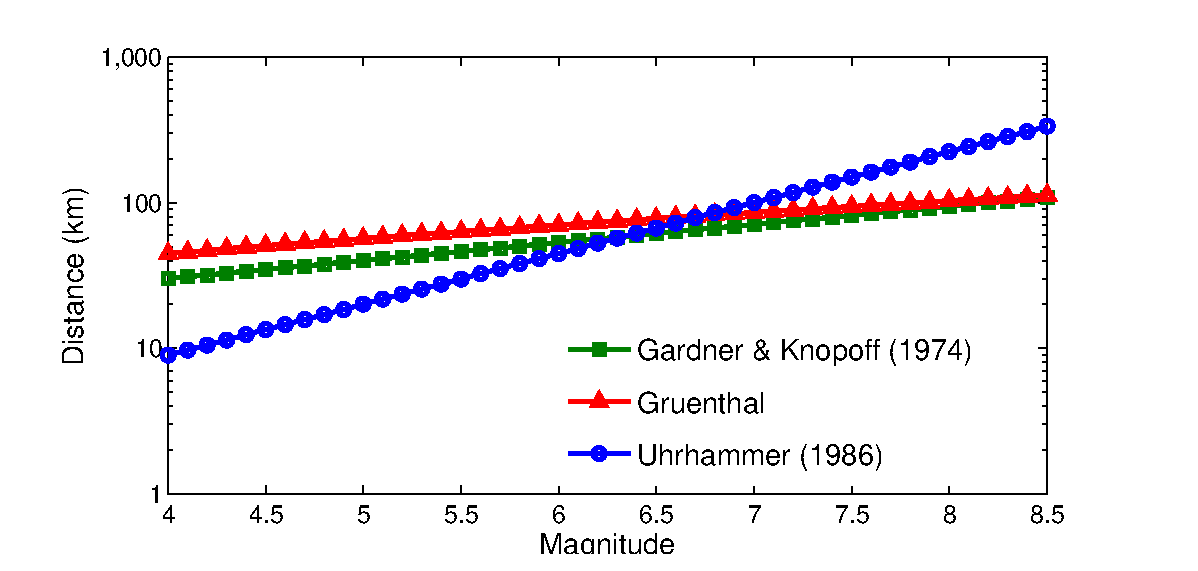
\includegraphics[width=8cm]{./figures/declustering_distance_windows.eps}
	\end{subcaption}
  \begin{subcaption}
      \centering
      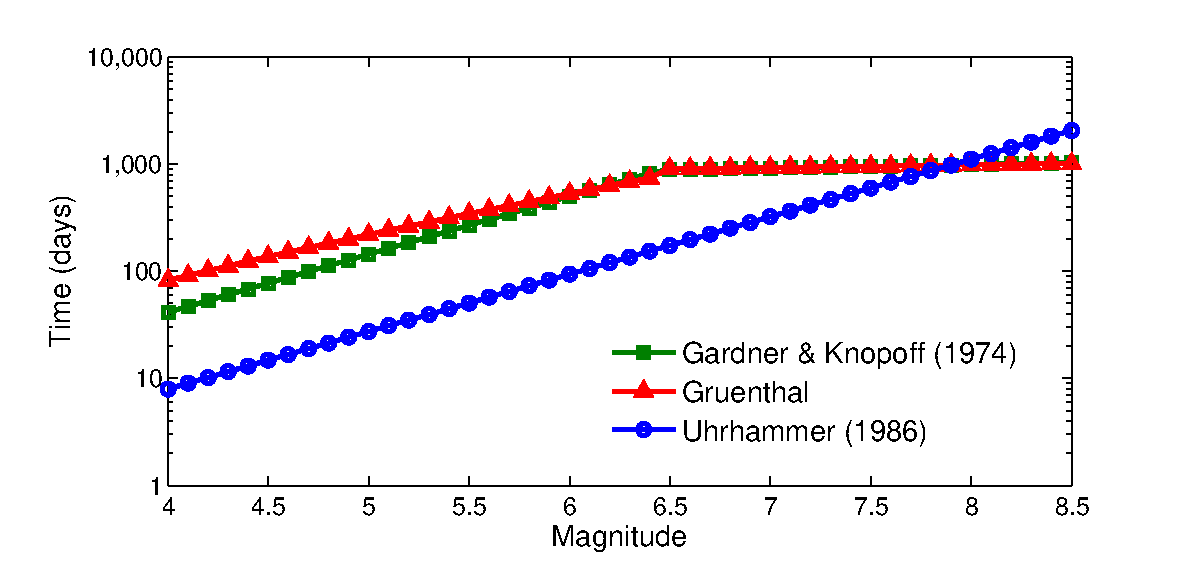
\includegraphics[width=8cm]{./figures/declustering_time_windows.eps}
	\end{subcaption}	
	\caption{Scaling of declustering time and distance windows with magnitude}
	\label{fig:declust_scaling}
\end{figure}

The \cite{GardnerKnopoff1974} algorithm and its derivatives represent 
are most computationally straightforward approach to declustering. The \verb=time_dist_windows= attribute indicates the choice of the 
time and distance window scaling model from the three listed. As 
the current version of this algorithm considers the events in a 
descending-magnitude order, the parameter \verb=foreshock_time_window= 
defines the size of the time window used for searching for foreshocks, 
as a fractional proportion of the size of the aftershock window (the 
distance windows are always equal for both fore- and aftershocks). 
So for an evenly sized time window for foreshocks and aftershocks, 
\verb=foreshock_time_window= should equal 1. For shorter or longer 
foreshock time windows this parameter can be reduced or increased respectively.

To run a declustering analysis on the earthquake catalogue it is necessary to set-up the configuration using a python dictionary.\footnote{A dictionary is Python's way of storing a mapping of data (including different types) to a set of keys (similar to a data structure in Matlab).} A config file for the \cite{GardnerKnopoff1974} algorithm, using for example the \cite{Uhrhammer1986} time-distance windows with equal sized time window for aftershocks and foreshocks, would be created as shown:

\begin{Verbatim}[frame=single, commandchars=\\\{\}, fontsize=\scriptsize, samepage=true]

In [1]: from hmtk.seismicity.declusterer.distance_time_windows import UhrhammerWindow

In [2]: declust_config = \{'time_distance_window': UhrhammerWindow(),
   ....:                   'fs_time_prop': 1.0\}

\end{Verbatim}


To run the declustering algorithm simply import and run the algorithm as shown:

\begin{Verbatim}[frame=single, commandchars=\\\{\}, fontsize=\scriptsize, samepage=true]

In [1]: from hmtk.seismicity.declusterer.distance_time_windows import UhrhammerWindow

In [2]: declust_config = \{'time_distance_window': UhrhammerWindow(),
   ....:                   'fs_time_prop': 1.0\}

\end{Verbatim}


\begin{Verbatim}[frame=single, commandchars=\\\{\}, fontsize=\scriptsize, samepage=true]

In [3]: from hmtk.seismicity.declusterer.dec_gardner_knopoff import GardnerKnopoffType1

In [4]: declustering = GardnerKnopoffType1()

In [5]: cluster_index, cluster_flag = declustering.decluster(catalogue,
                                                             declust_config)

\end{Verbatim}

There are two outputs of a declustering algorithm: \verb=cluster_index= and \verb=cluster_flag=. Both are numpy vectors, of the same length as the catalogue, containing information about the clusters in the catalogue. \verb=cluster_index= indicates the cluster to which each event is assigned (0 if not assigned to a cluster). \verb=cluster_flag= indicates whether an event is a non-Poissonian event, in which case the value is assigned to 1, or a mainshock, the value is assigned as 0. This output definition is the same for all declustering algorithms.

At this point the user may wish to either retain the catalogue in its current format, in which case they may wish to add on the clustering information into another attribute of the catalogue.data dictionary, or they may wish to purge the catalogue of non-Poissonian events. 

To simply add the clustering information to the data dictionary simply type:

\begin{Verbatim}[frame=single, commandchars=\\\{\}, fontsize=\scriptsize, samepage=true]

In [6]: catalogue.data['Cluster_Index'] = cluster_index
In [7]: catalogue.data['Cluster_Flag'] = cluster_flag

\end{Verbatim}
 
Alternatively, to purge the catalogue of non-Poissonian events:

\begin{Verbatim}[frame=single, commandchars=\\\{\}, fontsize=\scriptsize, samepage=true]

In [6]: mainshock_flag = cluster_flag == 0
In [7]: catalogue.purge_catalogue(mainshock_flag)

\end{Verbatim}


\subsection{AFTERAN (\cite{Musson1999PSHABalkan})}

A particular development of the standard windowing approach is introduced in the program AFTERAN \cite{Musson1999PSHABalkan}. This is a modification of the \cite{GardnerKnopoff1974} algorithm, using a moving time window rather than a fixed time window. In AFTERAN, considering each earthquake in order of descending magnitude, events within a fixed distance window are identified (the distance window being those suggested previously). These events are searched using a moving time window of T days. For a given mainshock, non Poissonian events are identified if they occur both within the distance window and the initial time window. The time window is then moved, beginning at the last flagged event, and the process repeated. For a given mainshock, all non-Poissonian events are identified when the algorithm finds a continuous period of T days in which no aftershock or foreshock is identified. 

The theory of the AFTERAN algorithm is broadly consistent with that of \cite{GardnerKnopoff1974}. This algorithm, whilst a little more computationally complex, and therefore slower, than the \cite{GardnerKnopoff1974} windowing approach, remains simple to implement. 

As with the \cite{GardnerKnopoff1974} function, the \verb=time_dist_window= attribute indicates the choice of the time and distance window scaling model. The parameter \verb=time_window= indicates the size (in days) of the moving time window used to identify fore- and aftershocks. The following example will show how to run the AFTERAN algorithm, using the  \cite{GardnerKnopoff1974} definition of the distance windows, and a fixed-width moving time window of 100 days.

  
\begin{Verbatim}[frame=single, commandchars=\\\{\}, fontsize=\scriptsize, samepage=true]

In [1] from hmtk.seismicity.declusterer.dec_afteran import Afteran

In [2]: from hmtk.seismicity.declusterer.distance_time_windows import GardnerKnopoffWindow   
 
In [3]: declust_config = \{'time_distance_window': GardnerKnopoffWindow(),
                          'time_window': 100.0\} 

In [4]: declustering = Afteran()

In [5]: cluster_index, cluster_flag = declustering.decluster(catalogue, declust_config)

\end{Verbatim}

 

%::::::::::::::::::::::::::::::::::::::::::::::::::::::::::::::::::::::::::::::::::::::::::::::::::::::::::::::::::::::::::::::::::::::::::::::::::::::::::::::

\section{Completeness}

In the earliest stages of processing an instrumental seismic catalogue to derive inputs for seismic hazard analysis, it is necessary to determine the magnitude completeness threshold of the catalogue. To outline the meaning of the term ''magnitude completeness'' and the requirements for its analysis as an input to PSHA, the terminology of \cite{MignanWoessner2012} is adopted. This defines the magnitude of completeness as the ''lowest magnitude at which 100 \% of the events in a space-time volume are detected (\cite{RydelekSacks1989, WoessnerWiemer2005})''. Incompleteness of an earthquake catalogue will produce bias when determining models of earthquake recurrence, which may have a significant impact on the estimation of hazard at a site. Identification of the completeness magnitude of an earthquake catalogue is therefore a clear requirement for the processing of input data for seismic hazard analysis.

It should be noted that this summary of methodologies for estimating completeness is directed toward techniques that can be applied to a ''typical'' instrumental seismic catalogue. We therefore make the assumption that the input data will contain basic information for each earthquake such as time, location, magnitude. We do not make the assumption that network-specific or station-specific properties (e.g., configuration, phase picks, attenuation factors) are known a priori. This limits the selection of methodologies to those classed as estimators of ''sample completeness'', which defines completeness on the basis of the statistical properties of the earthquake catalogue, rather than ''probability-based completeness'', which defines the probability of detection given knowledge of the properties of the seismic network (\cite{SchorlemmerWoessner2008}). This therefore excludes the methodology of (\cite{SchorlemmerWoessner2008}), and similar approaches such as that of \cite{Felzer2008}

The current workflows assume that completeness will be applied to the whole catalogue, ideally returning a table of time-varying completeness. The option to explore spatial variation in completeness is not explicitly supported, but could be accommodated by an appropriate configuration of the toolkit.

In the current version (July 2013) of the Modeller's Toolkit only the \cite{Stepp1971} methodology for analysis of catalogue completeness is implemented. Further methods are in development, and will be input in future releases.

%\subsection{User-defined Table}
%
%This is simply a filtering that will remove from further consideration any events outside of the completeness bounds defined by the user. The table represents the time variation in $M_C$ and can be input as a separate file (in comma-separated value format) in the following format.
%\begin{Verbatim}[frame=single, commandchars=\\\{\}, fontsize=\scriptsize]
%1990.0, 4.0\\
%1960.0, 5.0\\
%1900.0, 6.0\\
%1700.0, 7.0\\
%\end{Verbatim}
%
%The left-hand column represents the earliest year at which the earthquake is complete at the corresponding magnitude in the right-hand column. \\
%\textbf{Important: The values in the completeness file must be entered from most-recent to oldest!} 

\subsection{\cite{Stepp1971}}

This is one of the earliest analytical approaches to estimation of completeness magnitude. It is based on estimators of the mean rate of recurrence of earthquakes within given magnitude and time ranges, identifying the completeness magnitude when the observed rate of earthquakes above MC begins to deviate from the expected rate. If a time interval ($T_i$) is taken, and the earthquake sequence assumed Poissonian, then the unbiased estimate of the mean rate of events per unit time interval of a given sample is:

\begin{equation}
   \lambda = \frac{1}{n} \sum_{i = 1}^{n} T_i
\end{equation}

with variance $\sigma_{\lambda}^{2} = \lambda / n$. Taking the unit time interval to be 1 year, the standard deviation of the estimate of the mean is:

\begin{equation}
   \sigma_{\lambda} = \sqrt{\lambda} / \sqrt{T}
\end{equation}

where $T$ is the sample length. As the Poisson assumption implies a stationary process, $\sigma_{\lambda}$ behaves as $1/\sqrt{T}$ in the sub-interval of the sample in which the mean rate of occurrence of a magnitude class is constant. Time variation of $M_C$ can usually be inferred graphically from the analysis, as is illustrated in Figure \ref{fig:SteppFigExample1}. In this example, the deviation from the $1/\sqrt{T}$ line for each magnitude class occurs at around 40 years  for $4.5 < M < 5$, 100 years for $5.0  < M < 6.0$, approximately 150 years for $6.0 < M < 6.5$ and 300 years for $M > 6.5$. Knowledge of the sources of earthquake information for a given catalogue may usually be reconciled with the completeness time intervals.

\begin{figure}[htb]
	\centering
		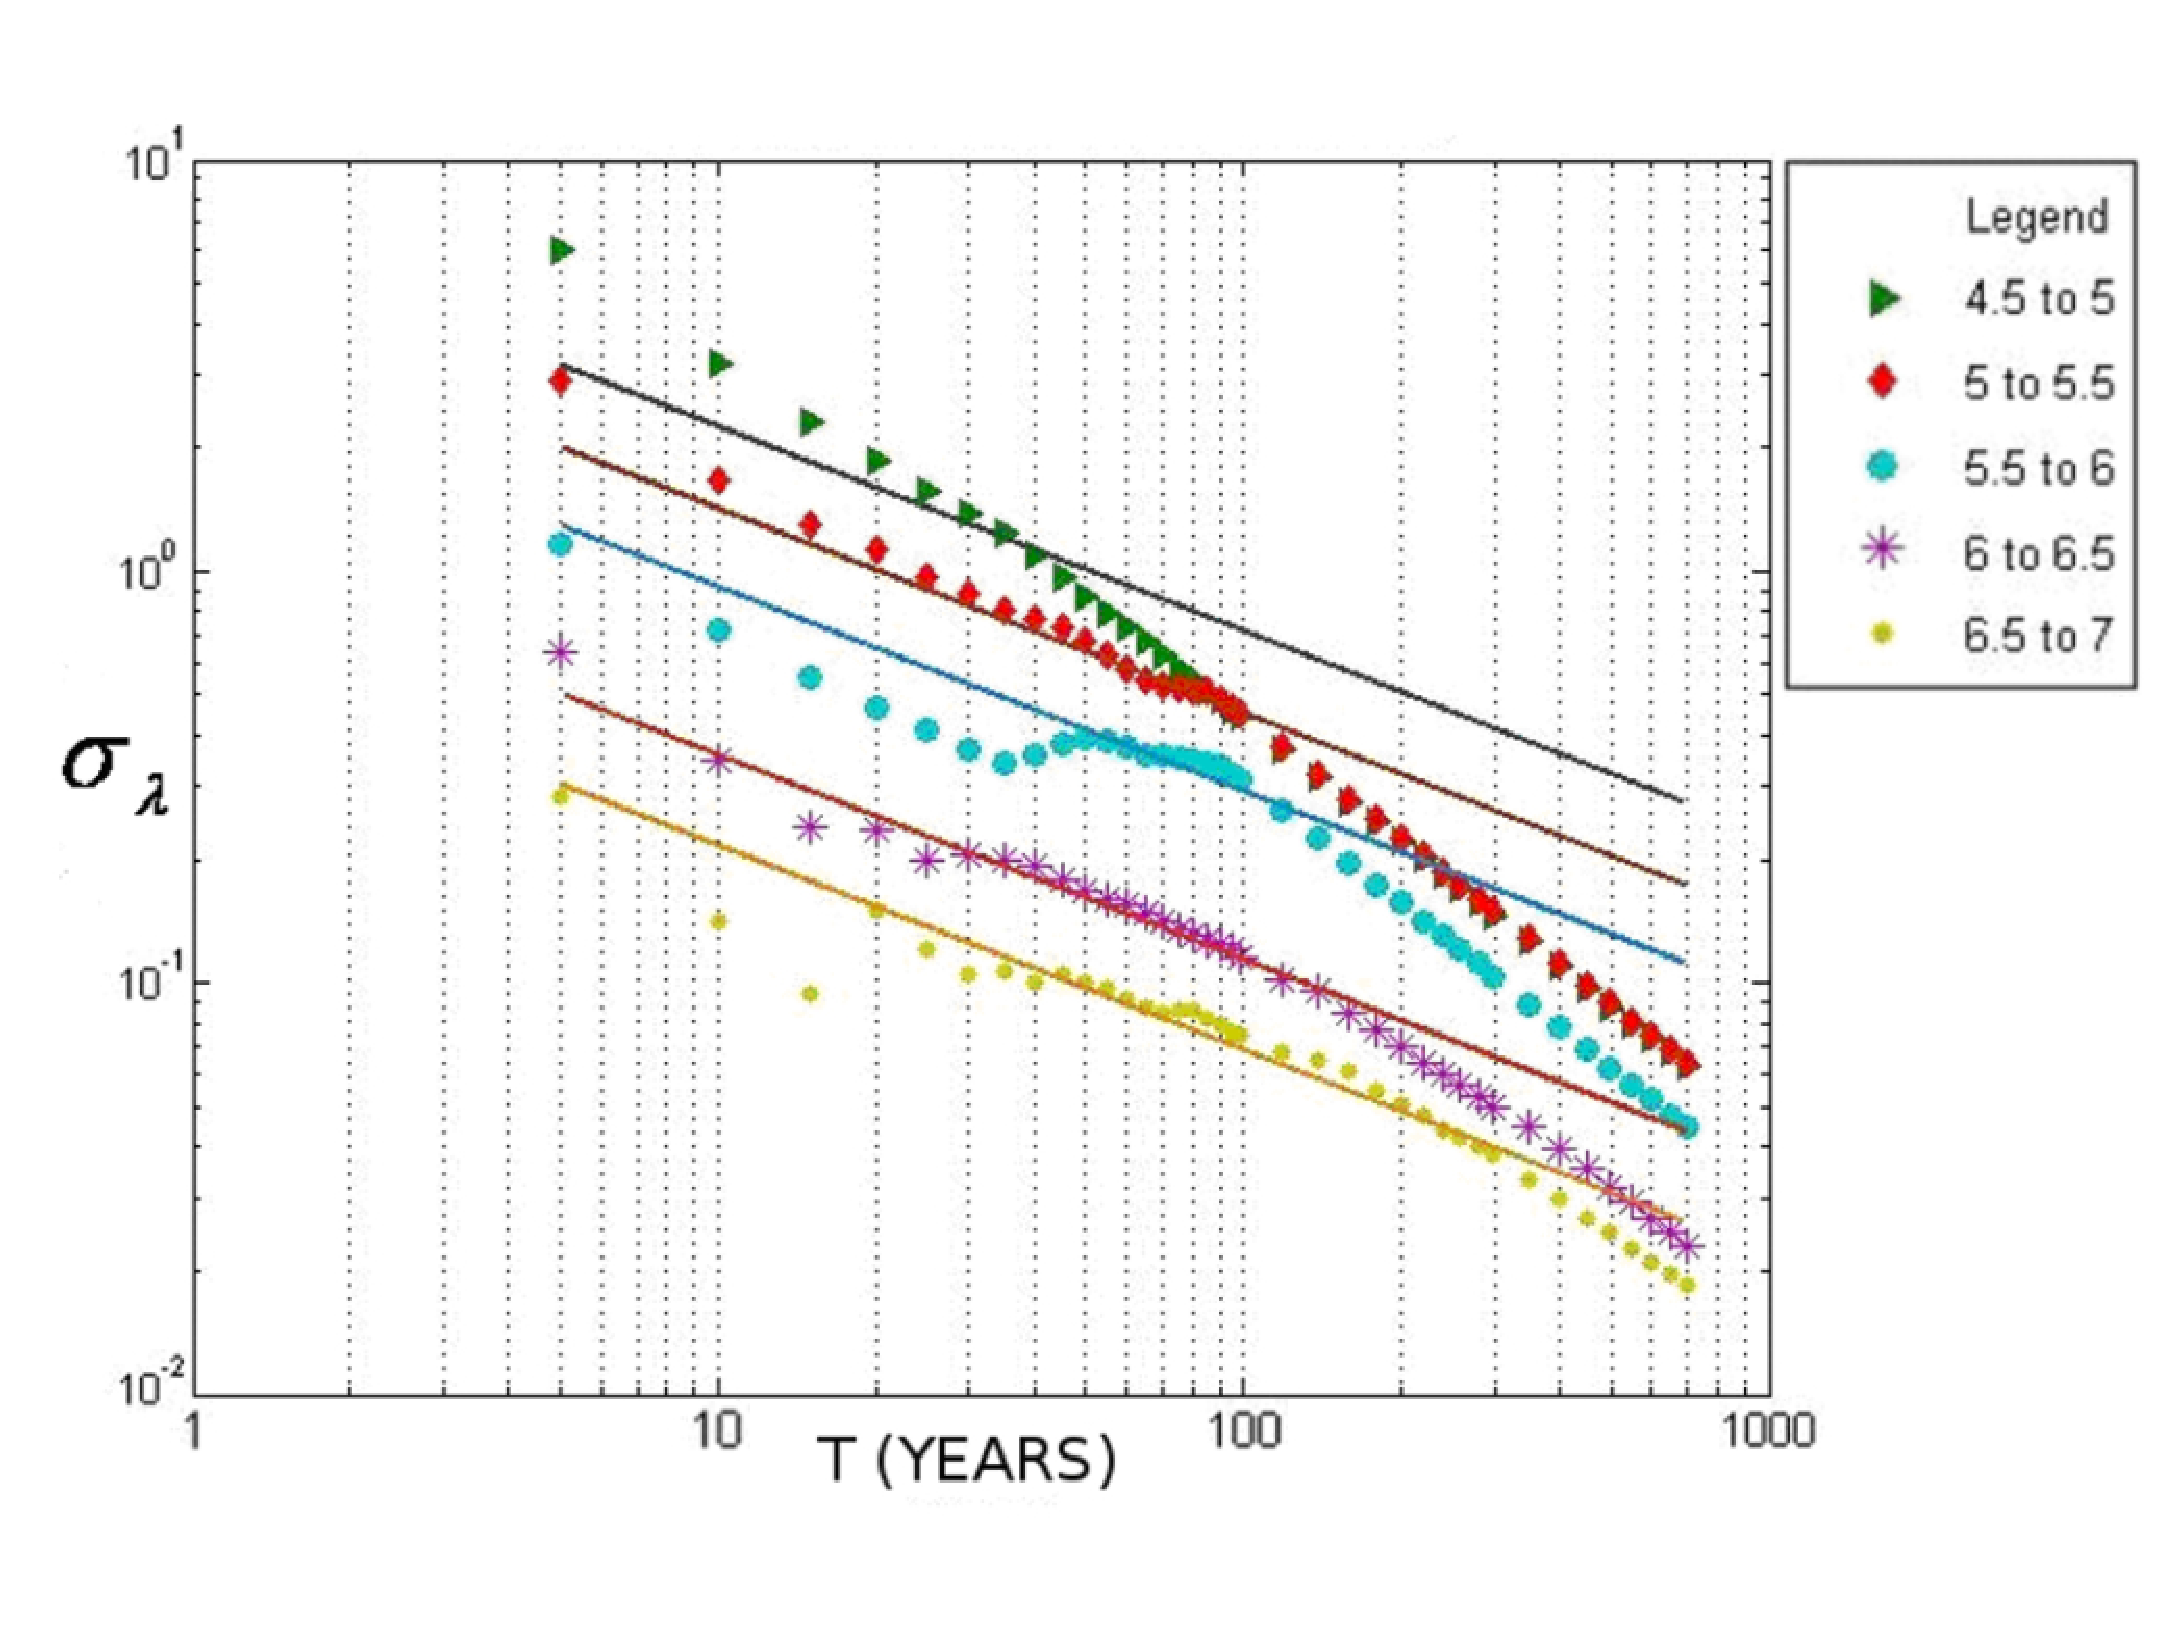
\includegraphics[height=10cm, keepaspectratio=true]{./figures/C2Fig1SteppFig1.eps}
	\caption{Example of Completeness Estimation by the \cite{Stepp1971} methodology}
	\label{fig:SteppFigExample1}
\end{figure}

The analysis of \citet{Stepp1971} is a coarse, but relatively robust, approach to estimating the temporal variation in completeness of a catalogue. It has been widely applied since its development. The accuracy of the completeness magnitude depends on the magnitude and time intervals considered, and a degree of judgement is often needed to determine the time at which the rate deviates from the expected values. It has tended to be applied to catalogues on a large scale, and for relatively higher completeness magnitudes. 

To translate the methodology from a largely graphical methods into a computational method the completeness period needs to be identified by automatically identifying the point at which the gradient of the observed values decreases with respect to that expected from a Poisson process (see \ref{fig:SteppFigExample1}). In the implementation found within the current toolkit, the divergence point is identified by fitting a two-segment piecewise linear function to the observed data. Although a two-segment piecewise linear function is normally fit with four parameters (intercept, $slope_1$, $slope_2$ and crossover point), by virtue of the assumption that for the complete catalogue the rate is assumed to be stationary such that $\sigma_{\lambda} = \frac{1}{\sqrt{T}}$ the slope of the first segment can be fixed as $-0.5$, and the second slope should be constrained such that $slope_2 \leq -0.5$, whilst the crossover point ($x_c$) is subject to the constraint ($x_c \geq 0.0$). Thus it is possible to fit the two-segment linear function using constrained optimisation with only three free parameters. For this purpose the toolkit minimises the residual sum-of-squares of the model fit using numerical optimisation. 

To run the \cite{Stepp1971} algorithm the configuration parameters should be entered in the form of a dictionary, such as the example shown below:

\begin{Verbatim}[frame=single, commandchars=\\\{\}, fontsize=\scriptsize, samepage=true]

In [1]: comp_config = \{'magnitude_bin': 0.5,
                        'time_bin': 5.,
                        'increment_lock': True\}

\end{Verbatim}

The algorithm has three configurable options. The \verb=time_bin= parameter describes the size of the time window in years, the \verb=magnitude_bin= parameter describes the size of the magnitude bin, sensitivity is as described previously. The final option (\verb=increment_lock=) is an option that is used to ensure consistency in the results to avoid the completeness magnitude increasing for the latest intervals in the catalogue simply due to the variability associated with the short duration. If \verb=increment_lock= is set to \verb=True=, the program will ensure that the completeness magnitude for shorter, more recent windows is less than or equal to that of older, longer windows. This is often a condition for some recurrence analysis tools, so it may be advisable to set this option to true in certain workflows. Otherwise it should be set to \verb=False to show the apparent variability=. Some degree of judgement is necessary here. In particular it is expected that the user may be aware of circumstances particular to their catalogue for which a recent increase in completeness magnitude is expected (for example, a certain recording network no longer operational).  


The process of running the algorithm is shown below:

\begin{Verbatim}[frame=single, commandchars=\\\{\}, fontsize=\scriptsize, samepage=true]

In [2]: from hmtk.seismicity.completeness.comp_stepp_1971 import Stepp1971

In [3]: completeness_algorithm = Stepp1971()

In [4]: completeness_table = completeness_algorithm.completeness(catalogue, comp_config)

In [5]: completeness_table
Out[5]: 
array([[ 1990.  ,     4.25],
       [ 1962.  ,     4.75],
       [ 1959.  ,     5.25],
       [ 1906.  ,     5.75],
       [ 1906.  ,     6.25],
       [ 1904.  ,     6.75],
       [ 1904.  ,     7.25]])

\end{Verbatim}

As shown in the resulting \verb=completeness_table=, the completeness algorithm will output the time variation in completeness (in this example with the \verb=increment_lock= set) in the form of a two-column table with column 1 indicating the completeness year for the magnitude bin centred on the magnitude value found in column 2.


At present, it may be the case that the user wishes to enter a time-varying completeness results for use in subsequent functions, based on alternative methods or on judgement. This can be entered in the \verb=completeness_table= setting, as in the example shown here (take note of the requirements for the square brackets):

\begin{Verbatim}[frame=single, commandchars=\\\{\}, fontsize=\scriptsize]

completeness_table: [[1990., 4.0],
                     [1960., 5.0],
                     [1930., 6.0],
                     [1900., 6.5]]

\end{Verbatim}

If a \verb=completeness_table= is input then this will override the selection of the completeness algorithm, and the calculation will take the values in \verb=completeness_table= directly. 

%::::::::::::::::::::::::::::::::::::::::::::::::::::::::::::::::::::::::::::::::::::::::::::::::::::::::::::::::::::::::::::::::::::::::::::::::::::::::::::::

\section{Recurrence Models}

The current sets of tools are intended to determine the parameters of the \cite{GutenbergRichter1944} recurrence model, namely the a- and b-value. It is expected that in the most common use case the catalogue that is input to these algorithms will be declustered, with a time-varying completeness defined according to a \verb=completeness_table= of the kind shown previously. If no \verb=completeness_table= is input the algorithm will assume the input catalogue is complete above the minimum magnitude for its full duration.

\subsection{\cite{Aki1965}}

The classical maximum likelihood estimator for a simple unbounded \cite{GutenbergRichter1944} model is that of \cite{Aki1965}, adapted for binned magnitude data by \cite{Bender1983}. It assumes a fixed completeness magnitude ($M_C$) for the catalogue, and a simple power law recurrence model. It does not explicitly take into account magnitude uncertainty.

\begin{equation}
   b = \frac{ \log_{10} \left( e \right)}{ \bar{m} - m_0 + \left( {\frac{\Delta M}{2}} \right)}
\end{equation}

\noindent where $\bar{m}$ is the mean magnitude, $m_0$ the minimum magnitude and $\Delta M$ the discretisation interval of magnitude within a given sample.

\subsection{Maximum Likelihood}

This method adjusts the \cite{Aki1965} and \cite{Bender1983} method to incorporate for time variation in completeness. The catalogue is divided into
into S sub-catalogues, where each sub-catalogue corresponds to a period 
with a corresponding $M_C$.  An average a- and b-value (with uncertainty) is returned by taking 
the mean of the a- and b-value of each sub-catalogue, weighted by 
the number of events in each sub-catalogue.

\begin{equation}
   \hat{b} = \frac{1}{S} \sum_{i = 1}^{S} w_i b_i
\end{equation}

\begin{Verbatim}[frame=single, commandchars=\\\{\}, fontsize=\scriptsize]

In [1]: mle_config = \{'magnitude_interval': 0.1,
                      'Average Type': 'Weighted',
                      'reference_magnitude': None\}

In [2]: from hmtk.seismicity.occurrence.b_maximum_likelihood import BMaxLikelihood

In [3]: recurrence = BMaxLikelihood()

In [4]: bval, sigmab, aval, sigmaa = recurrence.calculate(catalogue, mle_config, 
    completeness=completeness_table)

\end{Verbatim}

Where \verb=magnitude_window= indicates the size of the magnitude bin, \verb=recurrence_algorithm= and \verb=reference_magnitude= the magnitude for which the output calculates that rate greater than or equal to (set to \verb=0= for $10^{a}$). 

\subsection{\cite{KijkoSmit2012}}

A recent adaption of the \cite{Aki1965} estimator of b-value for  a catalogue containing different completeness periods has been proposed by \cite{KijkoSmit2012}. Dividing the earthquake catalogue into $s$ subcatalogues of $n_i$ events with corresponding completeness magnitudes $m_{c_i}$ for $i = 1, 2, ..., s$, the likelihood function of $\beta$ where $\beta = b \ln		 \left( {10.0} \right)$ is given as:

\begin{equation}
    \mathbf{L} = \prod_{i = 1}^{s} \prod_{j = 1}^{n_i} \beta \exp(\left[ {-\beta \left( {m_j^i - m_{min}^i } \right) } \right])
\end{equation}

which gives a maximum likelihood estimator of $\beta$:

\begin{equation}
    \beta = \left( {\frac{r_1}{\beta_1} + \frac{r_2}{\beta_2} + \dots + \frac{r_s}{\beta_s}} \right)^{-1}
\end{equation}

where $r_i = n_i / n$ and $n = \sum_{i = 1}^{s} n_i$ above the level of completeness $m_i$.

\begin{Verbatim}[frame=single, commandchars=\\\{\}, fontsize=\scriptsize]

In [1]: kijko_smit_config = \{'magnitude_interval': 0.1,
                             'reference_magnitude': None\}

\end{Verbatim}

\subsection{\cite{Weichert1980}}

Recognising the typical conditions of an earthquake catalogue, \cite{Weichert1980} developed a maximum likelihood estimator of $b$ for grouped magnitudes and unequal periods of observation. The likelihood formulation for this approach is:

\begin{equation}
   \mathbf{L} \left( {\beta | n_i, m_i, t_i} \right) = \frac{ N!}{\prod_i n_i!} \prod_i p_{i}^{n_i}
\end{equation}

where $\mathbf{L}$ is the likelihood estimator of $\beta$, $n$ the number of earthquakes in magnitude bin m with observation period t. The parameter $p$ is defined as:

\begin{equation}
   p_i = \frac{t_i \exp \left( {-\beta m_i} \right) }{\sum_j t_j \exp \left( {-\beta m_j} \right)}
\end{equation}

The extremum of $\ln \left( {\mathbf{L}}\right)$ is found at:

\begin{equation} 
   \frac{\sum_i t_i m_i \exp \left( {-\beta m_i} \right)}{\sum_j t_j \exp \left( {-\beta m_j} \right)}
\end{equation}

The computational implementation of this method is given as an appendix to \cite{Weichert1980}. This formulation of the maximum likelihood estimator for b-value, and consequently seismicity rate, is in widespread use, with applications in many national seismic hazard analysis \citep[e.g.]{usgsNSHM1996,usgsNSHM2002}. The algorithm has been demonstrated to be efficient and unbiased for most applications. It is recognised by \citet{Felzer2008} that an implicit assumption is made regarding the stationarity of the seismicity for all the time periods. 

To implement the \cite{Weichert1980} recurrence estimator, the configuration properties are defined as:

\begin{Verbatim}[frame=single, commandchars=\\\{\}, fontsize=\scriptsize]

In [1]: weichert_config = \{`magnitude_interval': 0.1,
                           `reference_magnitude': None,
                           \# The remaining parameters are optional
                           `bvalue': 1.0,
                           `itstab': 1E-5,
                           `maxiter': 1000\}

\end{Verbatim}

As the \cite{Weichert1980} algorithm is reaches the MLE estimation by iteration then three additional optional parameters can control the iteration process: \verb=bvalue= is the initial guess for the b-value, \verb=itstab= the difference in b-value in order to reach convergence, and \verb=maxiter= the maximum number of iterations. \footnote{The iterative nature of the \cite{Weichert1980} algorithm can result in very slow convergence and unstable behaviour when the magnitudes infer b-values that are very small, or even negative. This can occur when very few events are in the resulting catalogue, or when the magnitudes converge within a narrow range.}



%::::::::::::::::::::::::::::::::::::::::::::::::::::::::::::::::::::::::::::::::::::::::::::::::::::::::::::::::::::::::::::::::::::::::::::::::::::::::::::::
\section{Maximum Magnitude}

The estimation of the maximum magnitude for use in seismic hazard analysis is a complex, and often controversial, process that should be guided by information from geology and the seismotectonics of a seismic source. Estimation of maximim magnitude from the observed (instrumental and historical) seismicity can be undertaken using methods assuming a truncated \cite{GutenbergRichter1944} model, or via non-parametric methods that are independent any assumed functional form. 

\subsection{\cite{Kijko2004}}

Three different estimators of maximum magnitude are given by \cite{Kijko2004}, each depending on a different set of assumptions:
\begin{enumerate}
\item ''Fixed b-value'': Assumes a single b-value with no uncertainty 
\item ''Uncertain b-value'': Assumes and uncertain b-value defined by an expected b and the standard deviation
\item ''Non-Parametric Gaussian'': Assumes no functional form (can be applied to seismicity observed to follow a more characteristic distribution)
\end{enumerate}

Each of these estimators assumes the general form:

\begin{equation}
m_{max} = m_{max}^{obs} + \Delta
\end{equation}

where $\Delta$ is an increment that is dependent on the estimator used.

The uncertainty on $m_{max}$ is also defined according to:

\begin{equation}
    \sigma_{m_{max}} = \sqrt{\sigma_{m_{max}^{obs}}^2 + \Delta^{2}}
\end{equation}

In the three estimators some lower bound magnitude constraint must be defined. For those estimators that assume an exponential recurrence model the lower bound magnitude must be specified by the users. For the non-Parametric Gaussian method and explicit lower bound magnitude does not have to be specified; however, the estimation is conditioned upon the largest N magnitudes, where N must be specified by the user.

If the user wishes to input a maximum magnitude that is larger than that observed in the catalogue (e.g. a known historical magnitude), this can be specified in the config file using \verb=input_mmax= with the corresponding uncertainty defined by \verb=input_mmax_uncertainty=. If these are not defined (i.e. set to \verb=None=) then the maximum magnitude will be taken from the catalogue.

All three estimators require an iterative solution, therefore additional parameters can be specified in the configuration file that control the iteration process: \verb=tolerance= difference in $M_Max$ estimate for the algorithm to be considered converged, and \verb=maximum_iterations= the maximum number of iterations for stability. 


\subsubsection{''Fixed b-value''}

For a catalogue of $n$ earthquakes, whose magnitudes are distributed by a \cite{GutenbergRichter1944} distribiution with a fixed "b" value, the increment of maximum magnitude is determined via:

\begin{equation}
\Delta = \int\limits_{m_{min}} ^{m_{max}} \left[ {\frac{1 - \exp \left[ {-\beta \left( {m - m_{min}} \right)} \right]}{1 - \exp \left[ {-\beta \left( {m_{max}^{obs} - m_{min}} \right) } \right]}} \right] ^n dm
\end{equation}


The execution of the \cite{Kijko2004} ''fixed-b'' algorithm is as follows:

\begin{Verbatim}[frame=single, commandchars=\\\{\}, fontsize=\scriptsize]

In [1]: mmax_config = \{`input_mmax': 7.6,
                       `input_mmax_uncertainty': 0.22,
                       `b-value': 1.0,
                       `input_mmin': 5.0,
                       `tolerance': 1.0E-5,  \# Defaults to this if not specified
                       `maximum_iterations': 1000\} \# Defaults to this if not specified
                       
In [2]: from hmtk.seismicity.max_magnitude.kijko_sellevol_fixed_b import KijkoSellevolFixedb

In [3]: mmax_estimator = KijkoSellevolFixedb()

In [4]: mmax, mmax_uncertainty = mmax_estimator.get_mmax(catalogue, mmax_config)
                
\end{Verbatim}

\subsubsection{''Uncertain b-value''}

For a catalogue of $n$ earthquakes, whose magnitudes are distributed by a \cite{GutenbergRichter1944} distribiution with an uncertain "b" value, characterised by and expected term ($b$) and a corresponding undertainty ($\sigma_b$), the increment of maximum magnitude is determined via:


\begin{equation}
\Delta = \left( {C_{\beta}} \right)^n \int\limits_{m_min}^{m_max} \left[ {1 - \left( {\frac{p}{p + m - m_{min}}} \right) ^q} \right]^n dm
\end{equation}

where $\beta = b \ln \left( {10.0} \right)$, $p = \beta / \left( {\sigma_{\beta}} \right) ^ 2$, $q = \left( {\beta / \sigma_{\beta}} \right) ^ 2$ and $C_{\beta}$ is a normalising coefficient determined via:

\begin{equation}
C_{\beta} = \frac{1}{1 - \left[ {p / \left( {p + m_{max} - m_{min}} \right) } \right]^q}
\end{equation}

In both the fixed and uncertain ''b'' case a minimum magnitude will need to be input into the calculation. If this value is lower than the minimum magnitude observed in the catalogue the iterator may not stabilise to a satisfactory value, so it is recommended to use a minimum magnitude that is greater than the minimum found in the observed catalogue.

The execution of the ''uncertain b-value'' estimator is undertaken in a very similar to that of the fixed b-value, the only additional parameter being the \verb=sigma-b= term:

\begin{Verbatim}[frame=single, commandchars=\\\{\}, fontsize=\scriptsize]

In [1]: mmax_config = \{'input_mmax': 7.6,
                       'input_mmax_uncertainty': 0.22,
                       'b-value': 1.0,
                       'sigma-b': 0.15
                       'input_mmin': 5.0,
                       'tolerance': 1.0E-5, \# Defaults to this if not specified
                       'maximum_iterations': 1000\} \# Defaults to this if not specified
                       
In [2]: from hmtk.seismicity.max-magnitude.kijko_sellevol_bayes import KijkoSellevolBayes

In [3]: mmax_estimator = KijkoSellevolBayes()

In [4]: mmax, mmax_uncertainty = mmax_estimator.get_mmax(catalogue, mmax_config)
                
\end{Verbatim}

\subsubsection{Non-Parametric Gaussian}

The non-parametric Gaussian estimator for maximum magnitude $m_{max}$ is defined as:

\begin{equation}
\Delta = \int\limits_{m_{min}}^{m_{max}} \left[ {\frac{\sum_{i = 1}^{n} \left[ {\Phi \left( {\frac{m - m_i}{h}} \right) - \Phi \left( {\frac{m_{min} - m_i}{h}} \right)} \right]}{\sum_{i = 1}^{n} \left[ {\Phi \left( {\frac{m_{max} - m_i}{h}} \right) - \Phi \left( {\frac{m_{min} - m_i}{h}} \right)} \right]}} \right]^n  dm
\end{equation}
where $m_{min}$ and $m_{max}$ are the minimum and maximum magnitudes from a set of $n$ events, $\Phi$ is the standard normal cumulative distribution function. $h$ a kernel smoothing factor:
\begin{equation}
h = 0.9 \times min\left( {\sigma, IQR / 1.34} \right) \times n^{-1 / 5}
\end{equation}
with $\sigma$ the standard deviation of a set of n earthquakes with magnitude $m_{i}$ where $i = 1, 2, ... n$, and $IQR$ the inter-quartile range. 

Therefore the uncertainty on $m_{max}$ is conditioned primarily on the uncertainty of the largest observed magnitude. As in many catalogues the largest observed magnitude may be an earlier historical event, which will be associated with a large uncertainty, this estimator tends towards large uncertainties on $m_{max}$.

Due to the need to define some additional parameters the configuration file is slightly different. No b-value or minimum magnitude needs to be specified; however, the algorithm will consider only the largest \verb=number_earthquakes= magnitudes (or all magnitudes if the number of observations is smaller). The algorithm also numerically approximates the integral of the Gaussian pdf, so \verb=number_samples= is the number of samples of the distribution. The rest of the execution remains the same as for the exponential recurrence estimators of $M_{max}$:

\begin{Verbatim}[frame=single, commandchars=\\\{\}, fontsize=\scriptsize]

In [1]: mmax_config = \{'input_mmax': 7.6,
                       'input_mmax_uncertainty': 0.22,
                       'number_samples': 51, \# Default value
                       'number_earthquakes': 100 \# Default value
                       'tolerance': 1.0E-5, \# Defaults to this if not specified
                       'maximum_iterations': 1000\} \# Defaults to this if not specified
                       
In [2]: from hmtk.seismicity.max-magnitude.kijko_nonparametric_gausian import KijkoNonParametricGaussian

In [3]: mmax_estimator = KijkoNonParametricGaussian()

In [4]: mmax, mmax_uncertainty = mmax_estimator.get_mmax(catalogue, mmax_config)
                
\end{Verbatim}


\subsection{Cumulative Moment\citep{MakropoulosBurton1983}}

The cumulative moment release method is an adaptation of the cumulative strain energy release method for estimating $m_{max}$ originally proposed by \cite{MakropoulosBurton1983}. Another method based on a pseudo-graphical formulation, an estimator of maximum magnitude can be derived from a plot of cumulative seismic moment release with time. The average slope of this plot indicates the mean moment release for the input catalogue in question. Two further straight lines are defined with gradients equal to that of the slope of mean cumulative moment release, both enveloping the cumulative plot. The vertical distance between these two lines indicates the total amount of moment that may be released in the region, if no earthquakes were to occur in the corresponding time (i.e. the distance between the upper and lower bounding lines on the time axis). This concept is illustrated in Figure \ref{fig:Cumulative_Moment}. 

\begin{figure}[htb]
	\centering
		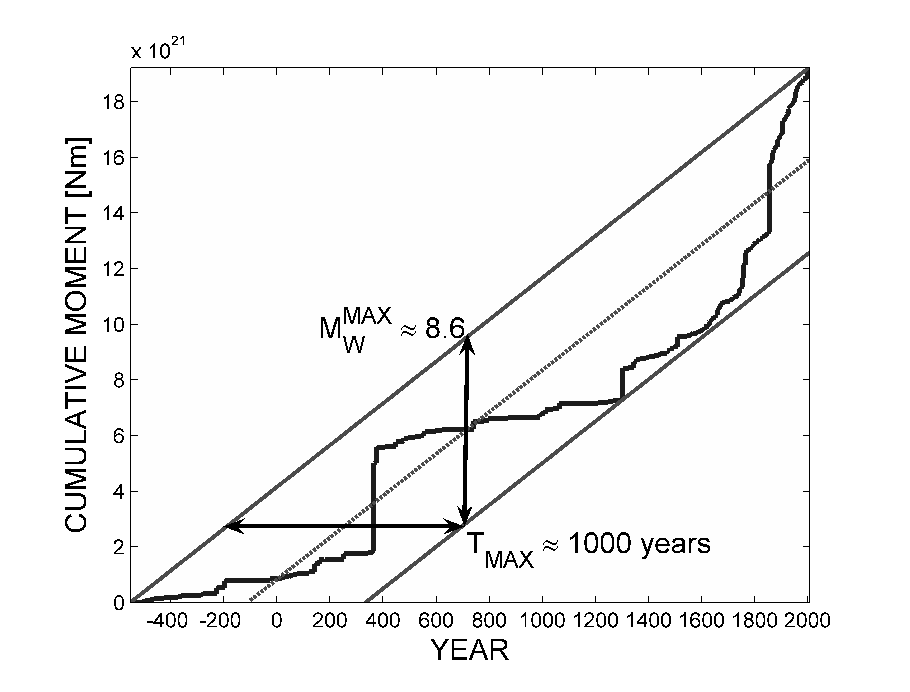
\includegraphics[height=6cm, keepaspectratio=true]{./figures/Cumulative_Moment.eps}
	\caption{Illustratation of Cumulative Moment Release Concept}
	\label{fig:Cumulative_Moment}
\end{figure}

The cumulative moment estimator of $m_{max}$, whilst simple in concept, has several key advantages. As a non-parametric method it is independent of any assumed probability distribution and cannot estimate $m_{max}$ lower than the observed $m_{max}$. It is also principally controlled by the largest events in the catalogue, this making it relative insensitive to uncertainties in completeness or lower bound threshold. In practice, this estimator, and to some extent that of \cite{Kijko2004} are dependent on having a sufficiently long record of events relative to the strain cycle for the region in question, such that the estimate of average moment release is stable. This will obviously depend on the length of the catalogue, and for some regions, particularly those in low strain intraplate environments, it is often the case that $m_{max}$ will be close to the observed $m_{max}$. Therefore it may be the case that it is most appropriate to use these techniques on a larger scale, either considering multiple sources or an appropriate tectonic proxy.

For the cumulative moment estimator it is possible to take into account the uncertainty on $m_{max}$ by applying bootstrap sampling to the observed magnitudes and their respective uncertainties. This has the advantage that $\sigma_{m_{max}}$ is not controlled by the uncertainty on the observed $m_{max}$, as it is for the \cite{Kijko2004} algorithm. Instead it takes into account the uncertainty on all the magnitudes in the catalogue. The cost of this, however, is that this method is more computationally intensive, and therefore slower, than \cite{Kijko2004}, depending on the number of bootstrap samples the user chooses.

The algorithm is slightly simpler to run than the \cite{Kijko2004} methods; however, due to the bootstrapping process it is slightly slower. It is run as per the following example:

\begin{Verbatim}[frame=single, commandchars=\\\{\}, fontsize=\scriptsize]

In [1]: mmax_config = {'number_bootstraps': 1000}
                       
In [2]: from hmtk.seismicity.max_magnitude.cumulative_moment_release import CumulativeMoment

In [3]: mmax_estimator = CumulativeMoment()

In [4]: mmax, mmax_uncertainty = mmax_estimator.get_mmax(catalogue, mmax_config)
                
\end{Verbatim}

For the cumulative moment algorithm the only user configurable parameter is the \verb=number_bootstraps=, which is the number of samples used during the bootstrapping process. 

\section{Smoothed Seismicity}

The use of smoothed seismicity in seismic hazard analysis has generally become a common way of characterising distributed seismicity, for which the seismogenic source are defined exclusively from the uncertain locations of observed seismicity. There are many different methods for smoothing the catalogue, adopting different smoothing kernels or making different correction factors to compensate for spatial and/or temporal completeness. 

\subsection{\cite{frankel1995}}

A smoothed seismicity method that has one of the clearest precedents for use in seismic hazard analysis is that of \cite{frankel1995}, originally derived to characterise the seismicity of the Central and Eastern United States as part of the 1996 National Seismic Hazard Maps of the United States. The method applies a simple isotropic Gaussian smoothing kernel to derive the expected rate of events at each cell $\tilde{n}_i$ from the observed rate $n_j$ of seismicity in a grid of $j$ cells. This kernel takes the form:

\begin{equation}
\tilde{n_i} = \frac{\sum_j n_j e^{d_{ij}^2 / c^2}}{\sum_j e^{d_{ij}^2 / c^2}} 
\end{equation}

In the implementation of the algorithm, two steps are taken that we prefer to make configurable options here. The first step is that the time-varying completeness is accounted for using a correction factor ($t_f$) based on the \cite{Weichert1980} method:

 \begin{equation}
 t_f = \frac{\sum_i e^{-\beta m_{c_i}}}{\sum_i T_i e^{-\beta m_{c_i}}} 
 \end{equation}
 
where $m_{c_i}$ the completeness magnitude corresponding to the mid-point of each completeness interval, and $T_i$ the duration of the completeness interval. The completeness magnitude bins must be evenly-spaced; hence, within the application of the progress a function is executed to render the input completeness table to one in which the magnitudes are evenly spaced with a width of 0.1 magnitude units. 

\subsection{Implementing the Smoothed Seismicity Analysis}

The smoothed seismicity separates out the core implementation (i.e. the gridding, counting and execution of the code) and the choice of kernel. An example of the execution process is as follows:

The first stage is to upload the catalogue into an instance of the catalogue class

\begin{Verbatim}[frame=single, commandchars=\\\{\}, fontsize=\scriptsize]

In [1]: input_file = 'path/to/input_file.csv'

In [2]: from hmtk.parsers.catalogue.csv_catalogue_parser import CsvCatalogueParser

In [3]: parser = CsvCatalogueParser(input_file)

In [4]: catalogue = parser.read_file()

\end{Verbatim}

Next setup the smoothing algorithm using and the corresponding kernel:

\begin{Verbatim}[frame=single, commandchars=\\\{\}, fontsize=\scriptsize]

# Imports the smoothed seismicity algorithm
In [5]: from hmtk.seismicity.smoothing.smoothed_seismicity import SmoothedSeismicity

# Imports the Kernel function
In [6]: from hmtk.seismicity.smoothing.kernels.isotropic_gaussian import IsotropicGaussian

# Grid limits should be set up as 
# [min_long, max_long, spc_long, min_lat max_lat, spc_lat, min_depth, max_depth,
# spc_depth]
In [7]: grid_limits = [0., 10., 0.1, 0., 10., 0.1, 0., 60., 30.]
# Assuming a b-value of 1.0
In [8]: smooth_seis = SmoothedSeismicity(grid_limits, use_3d=True, bvalue=1.0)

\end{Verbatim}

The smoothed seismicity function needs to be set up with three variables: i) the extent (and spacing) of the grid, ii) the choice to use 3D smoothing (i.e. distances are taken as hypocentral rather than epicentral) and iii) the input b-value. The extent of the grid can also be defined from the catalogue. If preferred the user need only specify the spacing of the longitude-latitude grid (as a single floating point value), then the grid will be defined by taking the bounding box of the earthquake catalogue and extended by the total smoothing length (i.e. the bandwidth (in km) multiplied by the maximum number of bandwidths). 

To run the smoothed seismicity analysis, the configurable parameters are: \verb=BandWidth= the bandwidth of the Gaussian kernel (in km), \verb=Length_Limit= the number of bandwidths considered as a maximum smoothing length, and \verb=increment= chooses whether to output the incremental a-value (for consistency with the original \cite{frankel1995} methodology) or the cumulative a-value (corresponding to the a-value of the Gutenberg-Richter model).


The algorithm requires two essential inputs (the earthquake catalogue and the config file), and three optional inputs:

\begin{itemize}
\item \verb=completeness_table= A table of completeness magnitudes and their corresponding completeness years (as output from the completeness algorithms)

\item \verb=smoothing_kernel= An instance of the required smoothing
kernel class (currently only Isotropic Gaussian is supported - and will be used if not specified)

\item \verb=end_year= The final year of the catalogue. This will be taken as the last year found in the catalogue, if not specified by the user
\end{itemize}

The analysis is then run via:

\begin{Verbatim}[frame=single, commandchars=\\\{\}, fontsize=\scriptsize]
# Set up config (e.g. 50 km band width, up to 3 bandwidths)
In [9]: config = {`Length_Limit': 3., `BandWidth': 50., 'increment': True}

# Run the analysis!
In [10]: output_data = smooth_seis.run_analysis(catalogue, config, completeness_table, smoothing_kernel=IsotropicGaussian(), end_year=None)

# To write the resulting data to a csv file
In [11] = smooth_seis.write_to_csv(`path/to/output_file.csv')
\end{Verbatim}

The resulting output will be a csv file with the following columns:
\begin{Verbatim}[frame=single, commandchars=\\\{\}, fontsize=\scriptsize]
Longitude, Latitude, Depth, Observed Count, Smoothed Rate, b-value
\end{Verbatim}

\noindent where \verb=Observed Count= is the observed number of earthquakes in each cell, and \\ 
\verb=Smoothed Rate= is the smoothed seismicity rate.







